\newpage
\section{Model-To-Tree with TGGs}
\genHeader

For those who have read Part IV, do you remember what one of the goals of using TGGs was? We hoped that, by specifying one direction of the transformation, we
could get the other free. That is exactly what's happened here! The final output of the forward transformation was the model specified in
\texttt{tree.xmi\_fwd.xmi}. This was used as input in the reverse transformation, whose final tree output is \texttt{tree.xmi\_FWD.xmi\_BWD.xmi}. If our
bidirectional transformation was successful, this tree should match the original text instance, \texttt{tree.xmi}. Let's compare the two.

\vspace{0.5cm}

\begin{figure}[htpb]
\begin{center}
  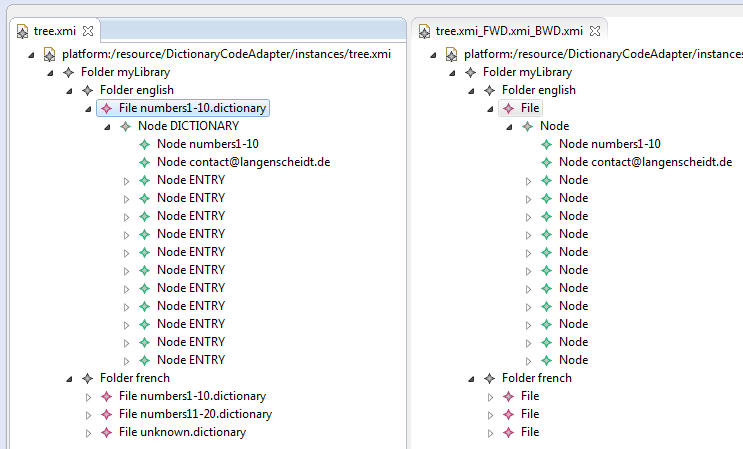
\includegraphics[width=\textwidth]{eclipse_generatedBackwardsModel}
  \caption{needs refinement\ldots}
  \label{eclipse:generatedBkwrdMdl}
\end{center}
\end{figure}

\vspace{0.5cm}

It's close, but not perfect. You can see that some things need to be refined. The ``DICTIONARY'' and ``ENTRY'' labels, for example, are missing from the
major nodes. You'll also notice that, as you scroll through each \texttt{Node}, the title and author have the correct \texttt{index} values of 0 and 1, but
unfortunately, \emph{every} other node is also set to 0. We need to bind each \texttt{entry} to a value so avoid potential conflicts when executing our TGG
transformation again, where our \texttt{NodeToDictionaryRule} assumes whatever node has this value must be the \texttt{authorNode}. Luckily, both of these are
very simple, quick fixes. We just need some more attribute constraints!

\jumpDual{m2tvis}{m2ttex}

\newpage
\hypertarget{m2tvis}{}
\subsection{Double-checking the TGG}
\visHeader

\begin{itemize}

\item[$\blacktriangleright$] Open \texttt{NodeToDictionaryRule} and update as depicted below (via attribute constraint). Is this in the right place? Should this
be done before??

\begin{figure}[htp]
\begin{center}
  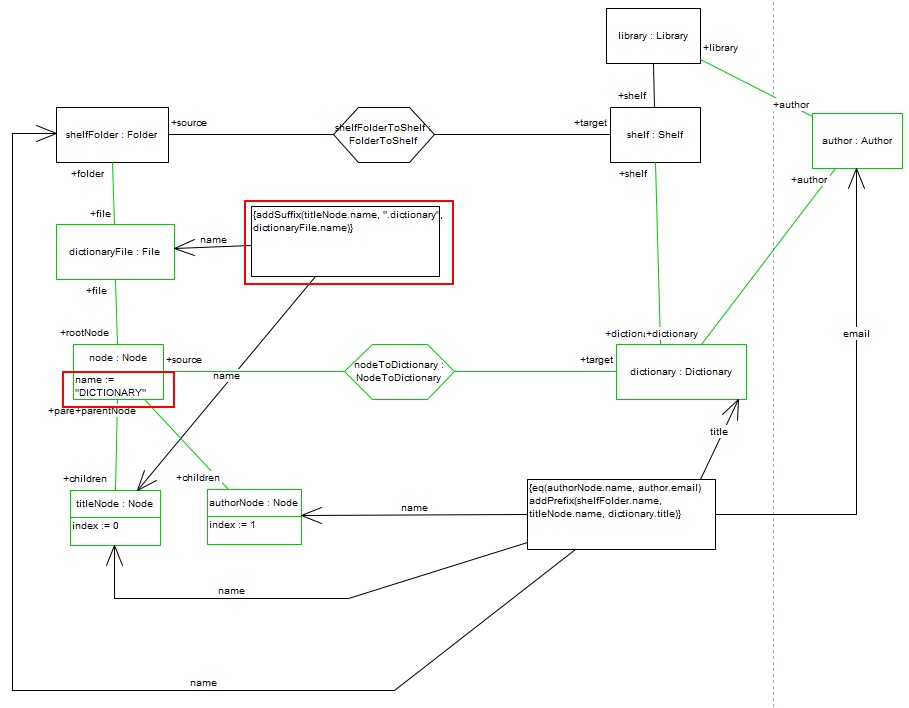
\includegraphics[width=\textwidth]{ea_updateNodeToDictionary}
  \caption{updated NodeToDictionary}
  \label{ea:NodeToDictionary_updated}
\end{center}
\end{figure}

\item[$\blacktriangleright$] Similarly, open \texttt{ForAllEntry} in EA and update like so:

\begin{figure}[htp]
\begin{center}
  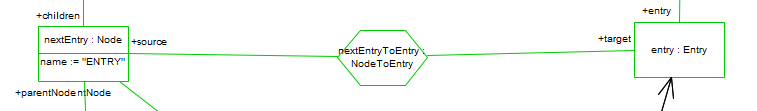
\includegraphics[width=\textwidth]{ea_updateForAllEntry}
  \caption{updated ForAllEntry}
  \label{ea:ForAllEntry_updated}
\end{center}
\end{figure}

\item[$\blacktriangleright$] End comment.

\jumpSingle{finalStep}

\end{itemize}


\newpage
\hypertarget{m2ttex}{}
\subsection{Refining the TGG Transformation}
\texHeader

\begin{itemize}

\item[$\blacktriangleright$] Find the relevant files and add the following attribute constraints. Note : the MOSL parser requires that all attribute constraints
are declared before link variables.

\begin{figure}[htp]
\begin{center}
  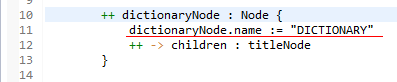
\includegraphics[width=0.8\textwidth]{eclipse_NodeToDictionaryRule_updated}
  \caption[labelInTOC]{needs refinement\ldots}
  \label{eclipse:generatedBkwrdMdl}
\end{center}
\end{figure}

\begin{figure}[htp]
\begin{center}
  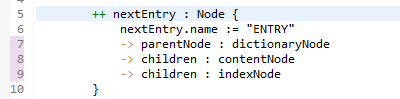
\includegraphics[width=0.8\textwidth]{eclipse_ForAllEntryRule_updated}
  \caption[labelInTOC]{needs refinement\ldots}
  \label{eclipse:generatedBkwrdMdl}
\end{center}
\end{figure} 

\item[$\blacktriangleright$] Add new SetDefaultNumber CSP here.

\begin{figure}[htbp]
\begin{center}
  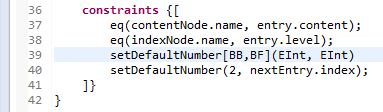
\includegraphics[width=0.6\textwidth]{eclipse_setDefaultNumberConstraint}
  \caption{extra constraint}
  \label{eclipse:newEntryConstraint}
\end{center}
\end{figure}

\end{itemize}


\newpage
\hypertarget{common cspConstraint}{}
\subsection{Implementing SetDefaultNumber}
\genHeader

We've declared and used our custom \texttt{SetDefaultNumber} constraint, but we haven't given it any implementation code yet. If you haven't yet, save and build
\texttt{DictionaryCodeAdapter} before continuing.

\begin{itemize}

\item[$\blacktriangleright$] Navigate to ``/src,'' where a new \texttt{csp.constraints} package was generated, and open \texttt{SetDefaultNumber.java}. Edit
this file until it matches Fig.~\ref{eclipse:setDefaultImpl}.

\begin{figure}[htbp]
\begin{center}
  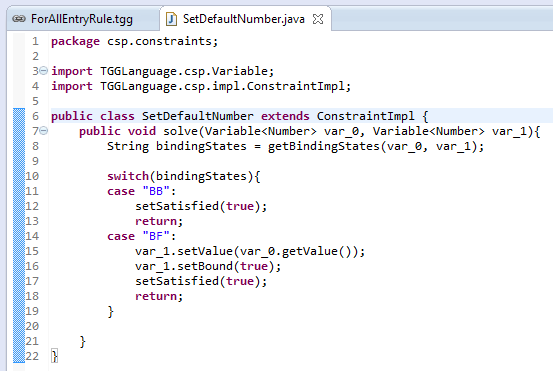
\includegraphics[width=0.9\textwidth]{eclipse_setDefaultNumberImplementation}
  \caption{extra constraint impl}
  \label{eclipse:setDefaultImpl}
\end{center}
\end{figure}

\item[$\blacktriangleright$] Save, build, and run \texttt{TGGMain} one more time. The inital and final \texttt{tree} variants should now be nearly identical! If
you're worried about some of the nodes being in the wrong order (such as an author at the bottom of the list), double-click on them and check their
\texttt{index} properties. If everything has been done correctly every \texttt{entry} should be 2, each \texttt{author} should be 1, and each \texttt{title}
should be 0.

\item[$\blacktriangleright$] On a final note to end the model-to-text step, wasn't it great how easy and short this was? If we were to use another
transformation set up (such as SDMs), we would have had to create independent rules for this backwards direction. Instead, TGGs gave us this transform for free!

\end{itemize}

